\documentclass{article}
\usepackage[utf8]{inputenc}
\usepackage[polish]{babel}
\usepackage[T1]{fontenc}
\usepackage{graphicx}
\usepackage{amsmath}
\usepackage{tikz}
\usepackage{mathdots}
\usepackage{yhmath}
\usepackage{cancel}
\usepackage{color}
\usepackage{siunitx}
\usepackage{array}
\usepackage{multirow}
\usepackage{amssymb}
\usepackage{gensymb}
\usepackage{tabularx}
\usepackage{booktabs}
\usepackage{multicol}
\usepackage{comment}
\usepackage{float}
\usetikzlibrary{fadings}
\usetikzlibrary{patterns}
\usetikzlibrary{shadows.blur}
\usetikzlibrary{shapes}


\title{ Zagraj w hokeja z ładunkami elektrycznymi \\
\large Dokumentacja}

\author{Kamil Sikora,
Maciej Ładoś,
Michał Bar}
\date{April 2020}

\begin{document}

\maketitle

\newpage
\tableofcontents

\newpage

\section{Opis projektu}
Projekt polega na symulacji gry w hokeja z dodatnio naładowanym krążkiem poruszanym jedynie poprzez wpływ innych ładunków elektrycznych. Gracz sam decyduje o rozmieszczeniu ładunków. Celem gry jest umieszczenie krążka w bramce. Gra kończy się po strzeleniu gola lub dotknięciu przez krążek któregoś z ładunków bądź przeszkód.\\
Projekt zdecydowaliśmy się wykonać w JavaScript

\section{Możliwości symulatora}

Aplikacja pozwala na śledzenie dokładnego zachowania ładunku w polu elektrycznym, jednocześnie udostępniając ciekawą rozgrywkę zachęcającą gracza do dokładniejszego prześledzenia interakcji wzajemnie oddziałujących między sobą ładunków. Lewy przycisk myszki dodaje ładunek ujemny we wskazane miejsce na planszy, a prawy dodatni.

Aby ułatwić wizualizację całego zachowania, możemy włączyć pole wektorowe które pozwoli nam zaobserwować siły działające na krążek w danym punkcie. Gracz może również po zaznaczeniu opcji 'Trace' rysować ślad poruszającego się krążka, a także z użyciem opcji 'Puck is positive' zmienić jego domyślny ładunek z dodatniego na ujemny.

Możemy również wyczyścić planszę, zatrzymać i wznowić grę, przywrócić krążek na pozycję startową, czy też zmienić masę krążka wpływając co zmienia siłę oddziaływania na niego przez ładunki.

\begin{figure}[H]
    \centering
    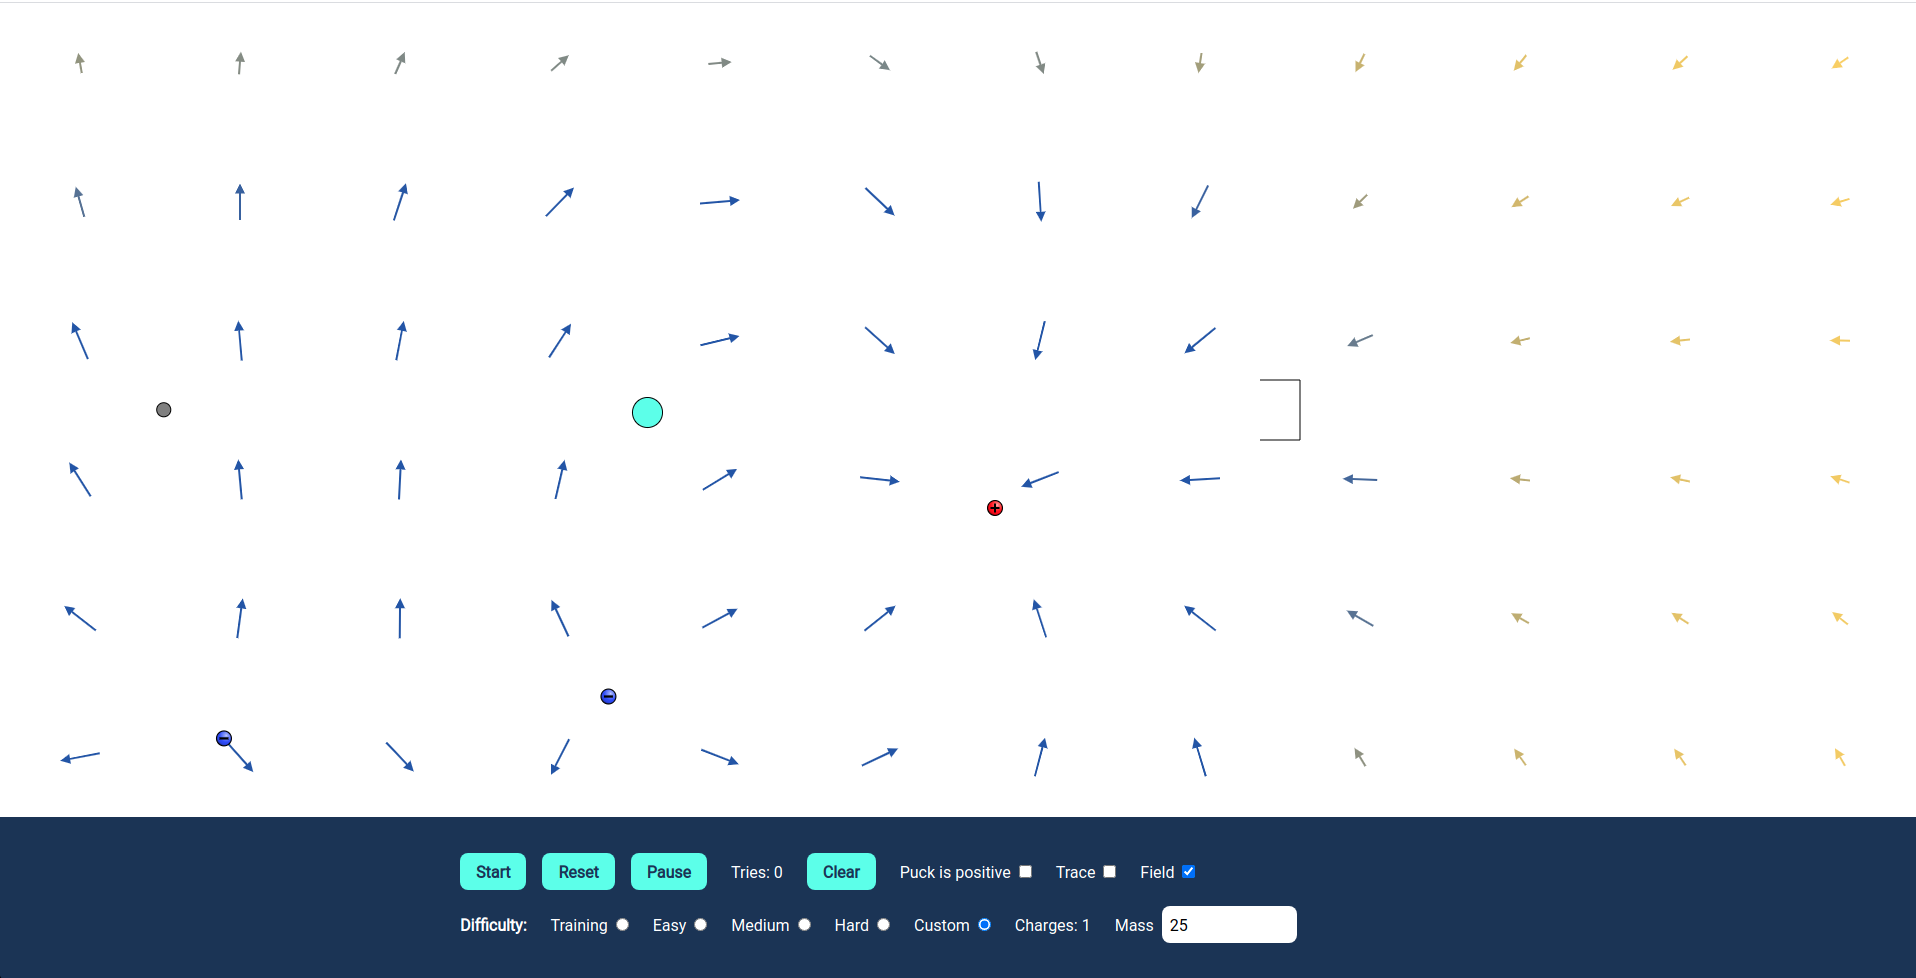
\includegraphics[width=\textwidth,height=\textheight,keepaspectratio]{img/field.png}
    \caption{Pole wektorowe, izotop}
    \label{fig:vector_drawing}
\end{figure}

Dla urozmaicenia i utrudnienia zabawy, użytkownikowi udostępnione zostały poziomy różnicujące poziom rozgrywki. Przeszkody w nich zawarte blokują przebieg krążka, i w razie ich dotknięcia kończy się rozgrywka. Poziom 'Custom' dodaje jeszcze specjalny obiekt - izotop, który emituje ładunki w losowej chwili i o zmiennym kierunku zmieniając tym samym rozkład sił na planszy i tym samym jeszcze bardziej wzbogacając zabawę. 

\begin{figure}[H]
    \centering
    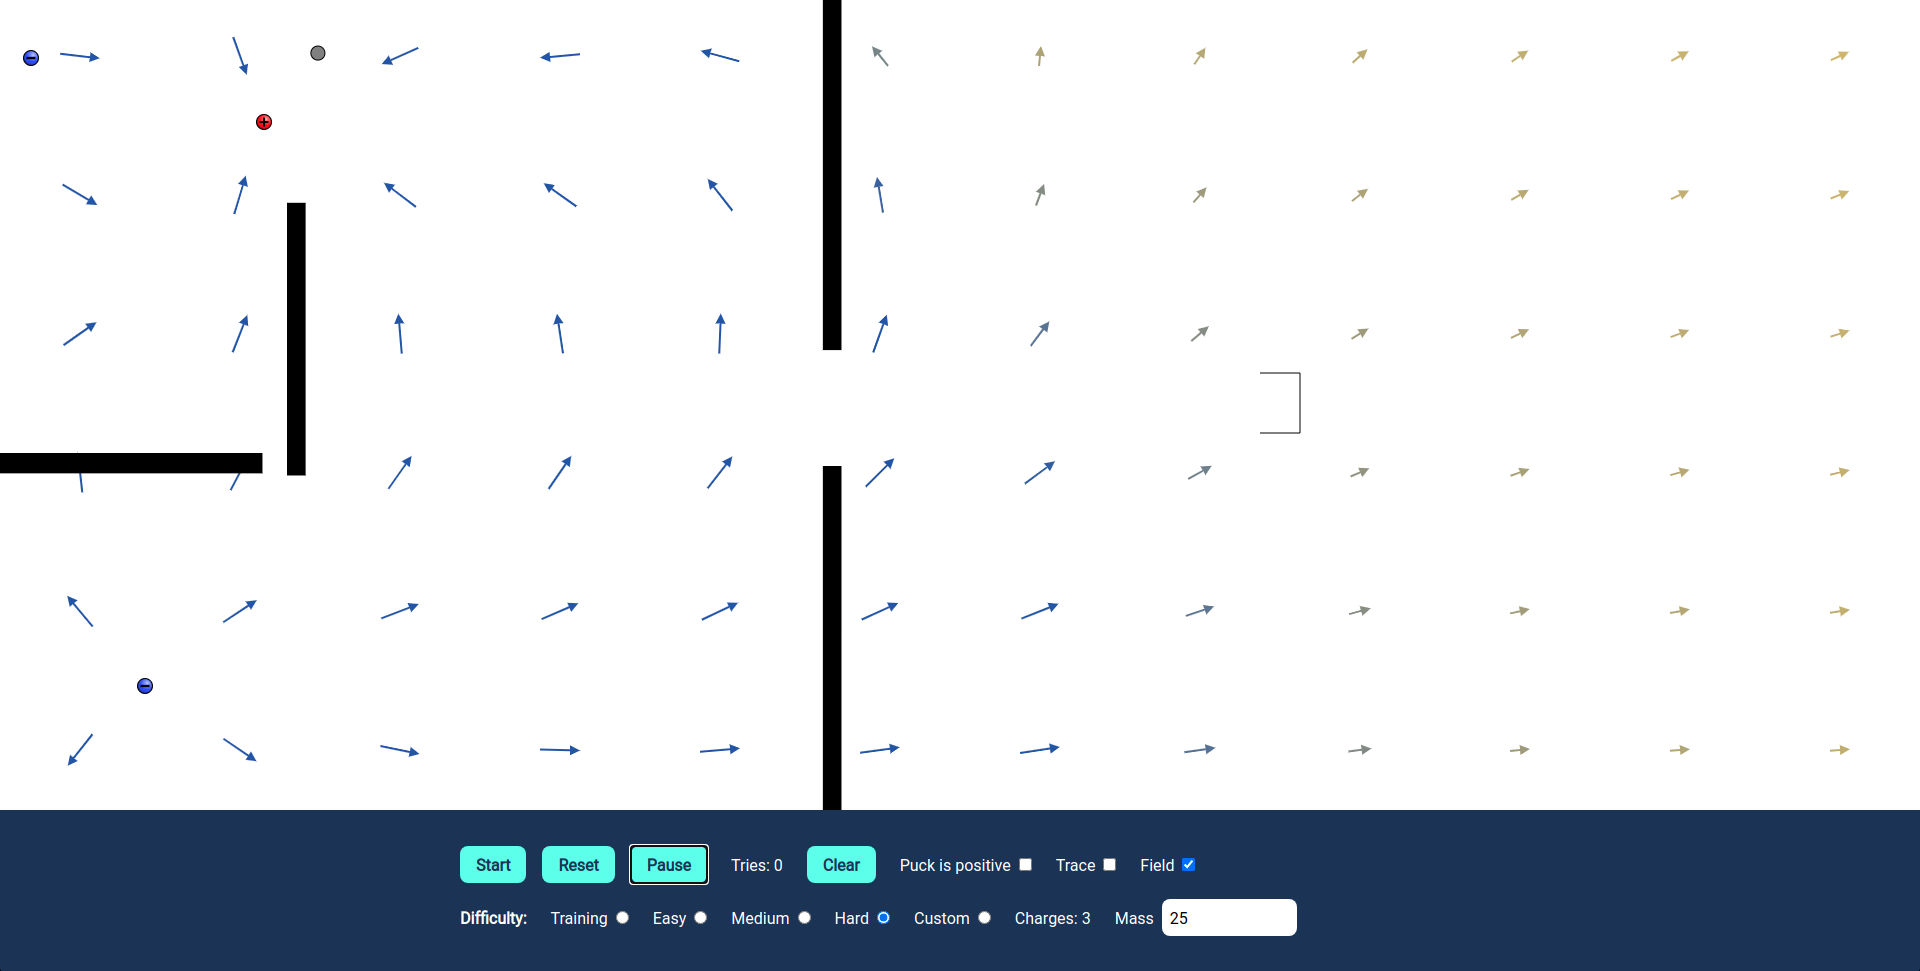
\includegraphics[width=\textwidth,height=\textheight,keepaspectratio]{img/level.png}
    \caption{Poziom z przeszkodami}
    \label{fig:vector_drawing}
\end{figure}


\section{Model fizyczny}
Fizyka w grze jest oparta na prawie Coulomba, którego treść brzmi: Siła wzajemnego oddziaływania dwóch naładowanych cząstek jest wprost proporcjonalna do iloczynu wartości tych ładunków i odwrotnie proporcjonalna do kwadratu odległości między nimi.


$$F=k \frac{q 1 \cdot q 2}{r^{2}}$$
$F$ - siła elektrostatyczna \\
$q1, q2$ - ładunki elektryczne \\
$r$ - odległość \\
$k$ - stała elektrostatyczna w przybliżeniu równa $9 \cdot 10^9 \frac{N \cdot m^2}{C^2}$
\\

\noindent Oba ładunki mają również masę, lecz w świecie cząstek, atomów i cząsteczek chemicznych, możemy całkowicie zaniedbać ich wzajemne oddziaływania grawitacyjne.


\begin{figure}[h]
    \centering
    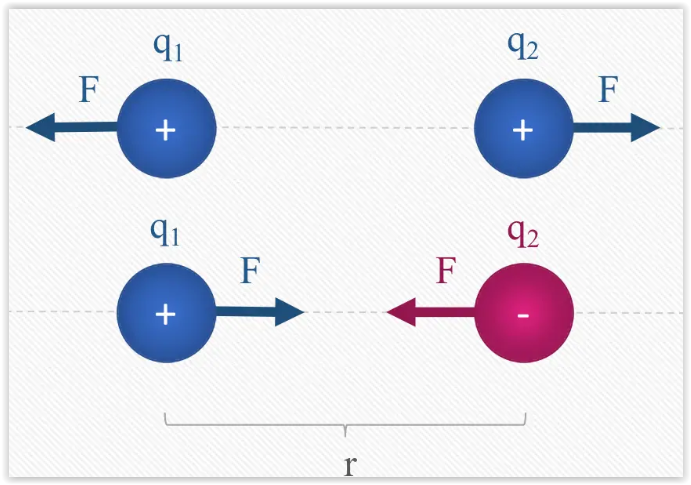
\includegraphics[scale=0.5]{img/Prawo_Coulomba.PNG}

    \caption{Prawo Coulomba- oddziaływanie ładunków}
    \label{fig:Prawo_Coulomba}
\end{figure}

\clearpage

\section{Model symulacyjny}

Nasza symulacja operuje w płaszczyźnie dwuwymiarowej. Każdy obiekt będzie posiadał dwie współrzędne - $x$ i $y$. Odległość między ciałami może być zatem wyznaczona jako odległość punktów na płaszczyźnie.

$$
r=\sqrt{\left(x_{b}-x_{a}\right)^{2}+\left(y_{b}-y_{a}\right)^{2}}
$$

\noindent W celu uproszczenia obliczeń siłę $\vec{F}$ oddziałującą na ładunki rozkładamy na składowe $\vec{F_x}$ oraz $\vec{F_y}$. Zakładamy, że środkiem naszego układu współrzędnych będzie krążek -- pozwoli nam to na skorzystanie z funkcji trygonometrycznych do wyliczenia tych składowych.

\tikzset{every picture/.style={line width=0.75pt}} %set default line width to 0.75pt

\tikzset{every picture/.style={line width=0.75pt}} %set default line width to 0.75pt        

\begin{center}
\begin{tikzpicture}[x=0.75pt,y=0.75pt,yscale=-1,xscale=1]
%uncomment if require: \path (0,261); %set diagram left start at 0, and has height of 261


%Shape: Right Triangle [id:dp36130500270564525] 
\draw   (387,62) -- (521.5,219) -- (387,219) -- cycle ;
%Straight Lines [id:da4371175600607653] 
\draw    (387,62) -- (387,216) ;
\draw [shift={(387,219)}, rotate = 270] [fill={rgb, 255:red, 0; green, 0; blue, 0 }  ][line width=0.08]  [draw opacity=0] (8.93,-4.29) -- (0,0) -- (8.93,4.29) -- cycle    ;
%Straight Lines [id:da010907474739860756] 
\draw  [dash pattern={on 4.5pt off 4.5pt}]  (387,62) -- (519.5,62.42) ;
\draw [shift={(522.5,62.43)}, rotate = 180.18] [fill={rgb, 255:red, 0; green, 0; blue, 0 }  ][line width=0.08]  [draw opacity=0] (8.93,-4.29) -- (0,0) -- (8.93,4.29) -- cycle    ;
%Straight Lines [id:da31420475263437164] 
\draw    (387,62) -- (519.55,216.72) ;
\draw [shift={(521.5,219)}, rotate = 229.41] [fill={rgb, 255:red, 0; green, 0; blue, 0 }  ][line width=0.08]  [draw opacity=0] (8.93,-4.29) -- (0,0) -- (8.93,4.29) -- cycle    ;

% Text Node
\draw (463,115) node [anchor=north west][inner sep=0.75pt]   [align=left] {$\displaystyle r$};
% Text Node
\draw (383,38) node [anchor=north west][inner sep=0.75pt]   [align=left] {$\displaystyle k$};
% Text Node
\draw (523.5,222) node [anchor=north west][inner sep=0.75pt]   [align=left] {$\displaystyle s$};
% Text Node
\draw (448,228) node [anchor=north west][inner sep=0.75pt]   [align=left] {$\displaystyle y$};
% Text Node
\draw (365,132.4) node [anchor=north west][inner sep=0.75pt]    {$x$};
% Text Node
\draw (361,181.4) node [anchor=north west][inner sep=0.75pt]    {$\vec{F}_{x}$};
% Text Node
\draw (493,30.4) node [anchor=north west][inner sep=0.75pt]    {$\vec{F}_{y}$};
% Text Node
\draw (411,65) node [anchor=north west][inner sep=0.75pt]   [align=left] {$\displaystyle \alpha $};
% Text Node
\draw (519,182.4) node [anchor=north west][inner sep=0.75pt]    {$\vec{F}$};

\end{tikzpicture}
\end{center}

\noindent Korzystając z funkcji trygonometrycznych otrzymamy:

$$
\sin \alpha=\frac{\vec{F}_{x}}{r}=\frac{x}{r} \quad \quad \cos \alpha=\frac{\vec{F}_{y}}{r}=\frac{y}{r}
$$

\noindent Przyjmujemy, że wartości ładunków są takie same, więc pomijamy je w obliczeniach. Wyprowadzamy wzory na składowe:

$$
\vec{F}_{x}=\frac{\sin \alpha}{r^{2}} \quad \vec{F}_{y}=\frac{\cos \alpha}{r^{2}}
$$

\noindent Korzystając z II zasady dynamiki Newtona, wyprowadzamy wzór na przyspieszenie ładunku:

$$
F=m \cdot a \Rightarrow a=\frac{F}{m}
$$

\noindent Ostatecznie wzory:

$$
a_{x}=k \cdot \frac{\sin \alpha}{m \cdot r^{2}} \quad a_{y}=k \cdot \frac{\cos \alpha}{m \cdot r^{2}}
$$

\section{Opis gry}
Celem gry jest umieszczenie krążka w bramce za pomocą wstawiania odpowiednich ładunków i w ten sposób generowania pola elektrycznego. Za pomocą prawego przycisku myszy wstawiamy ładunki dodatnie, a za pomocą lewego ujemne. Znak krążka który domyślnie jest ujemny możemy zmienić zaznaczając/odznaczając pole 'Puck is positive'. Dostępne są cztery poziomy trudności do wyboru: training, easy, medium, hard. Różnią się one ilością i rozmieszczeniem przeszkód.
W grze dostępne mamy przyciski do zarządzania akutalnym stanem planszy. 'Start' i 'Stop' służą rozpoczynania i zatrzymywania symulacji, 'Reset' ustawia pozycję krążka na domyślną, 'Clear' usuwa ładunki i ustawia pozycję krążka na domyślną. Licznik 'Tries' to ilość naszych błędnych prób, 'Charges' to ilość ładunków na planszy. Istnieje możliwość narysowania trasy przebytej przez krążek za pomocą pola 'Trace' oraz sił pola wektorowego za pomocą pola 'Field'. 

\section{Implementacja i architektura}
Kontrola rozgrywki realizowana jest z głównej klasy 'Game'. Zajmuje się ona inicjalizacją i kontrolą poszczególnych komponentów aplikacji. W niej zawarte są grupy obiektów, realizowany jest rendering sceny, a także na bieżąco sprawdzane są warunki rozgrywki. Dostarcza również podstawowych mechanizmów związanych z grą - przeliczania sił, definicji poziomów, czy komunikacją między elementami gry.

Następnie, implementując klasy obiektów, zawieramy w nich ich logikę oraz wygląd na planszy. Korzystając ze specjalnej magistrali wiadomości dostarczonej przez główną klasę gry, wszystkie obiekty (również sama gra) mogą wpływać na siebie i informować o różnych zdarzeniach. Rejestrując odpowiednie odpowiedzi na zdarzenia, sterujemy stanem gry, i decydujemy o podjęciu akcji na bazie aktywności gracza.

\subsection{Struktura kodu}
\begin{enumerate}
    \item const - folder zawiera pliki przechowujące wszelkie stałe wykorzystywane w programie
    \item assets - folder z plikami graficznymi oraz plikiem css
    \item controllers - są tu zawarte klasy obsługujące interakcje klienta z programem oraz akcje wykonywane przez program
    \item events - zawiera klasę która zapewnia obsługę zdarzeń w grze
    \item extensions - folder z rozszerzeniami wykorzystywanymi w programie
    \item models - zawarte są tu wszelkie klasy tworzące obiekty w grze oraz podfolder physics, który przechowuje obiekty fizyczne oraz model fizyczny
\end{enumerate}
\subsection{Wybrane stałe}
\begin{enumerate}
    \item COULOMB\_FORCE\_FACTOR - odpowiada stałej k z obliczeń z sekcji 'Model Symulacyjny'
    \item CHARGE\_MIN\_DISTANCE - minimalna odległość na jakiej utrzymywane są ładunki, aby nie dopuścić do współistnienia krążka i ładunku w tym samym miejscu i czasie zgodnie z zasadą Pauliego. W związku z tym zakładamy w naszym modelu dystans między ładunkami na minimum 25 jednostek odległości
    \item PUCK\_VELOCITY\_DIVIDER - dzielnik prędkości aby wizualizacja symulacji była lepiej dostrzegalna
\end{enumerate}

\clearpage
\subsection{Wybrane modele i ich metody}
\begin{enumerate}
    \item BoundingBox - główna klasa zapewniająca ruch oraz kolizje obiektów na planszy.
    Jej pola to \textit{x,y} składowe położenia oraz szerokość \textit{width} i wysokość \textit{height} obiektu.
    
    Zawiera trzy metody do obsługi kolizji: \textit{touches(), contains(), intersects()}.
    
    \textit{move()} przypisuje nowe położenie obiektu na podstawie przekazanych parametrów dotyczących przemieszczenia.
    
    \textit{distance()} oblicza dystans między obiektami w grze.
    
    \item GameObject - rozszerza \emph{BoundingBox}, bazowa abstrakcyjna klasa dla wielu modeli w grze. Deklaruje metody \textit{update(), render()}.
    \item Group - klasa implementująca działania na tablicach obektów tworzonych jako grupy w grze
    \item HockeyGoal - klasa implementująca rysowanie bramki na podstawie tworzonego \emph{BoundingBoxa}
    \item Obstacle - klasa dzięki która tworzy i renderuje przeszkody w grze
    \item Trace - klasa wykorzystywana przez klasę \textit{Puck} do rysowania trasy krążka
    \item ElectricCharge - bazowa klasa dla klas \textit{NegativeCharge, PositiveCharge} tworząca odpowiedni ładunek na podstawie przekazanego typu \emph{type}.\\
    Typ jest zawarty domyślnie w konstruktorach klas \textit{NegativeCharge, PositiveCharge}.
    \item Puck - klasa dziedzicząca po \emph{ElectricCharge} tworząca krążek jako ładunek ujemny lub dodatni.\\
    Krążek posiada własną masę \emph{mass} oraz promień \emph{radius}.
    
    \emph{acceleration, velocity} to odpowiednio przyspieszenie i prędkość krążka potrzebne do wyznaczania jego ruchu.
    
    \emph{trace} gdzie przypisany jest obiekt klasy \emph{Trace}  oraz \emph{traceIsActive} dotyczą możliwości rysowania przebytej przez krążek trasy.
    
   \textit{update(), render()} zapewniają odpowiednio ruch oraz rysowanie krążka.
   
   \clearpage
    \item VectorField - klasa tworząca obiekty składające się na pole wektorowe. Posiada ona ustalony zbiór punktów, i dla każdego z nich oblicza siłę która działałaby na krążek w danym miejscu. Następnie dla koordynatów tworzony jest obiekt \emph{FieldVector}, który rysowany jest na bazie przekazanej mu siły. Klasa pola wektorowego oblicza również medianę wszystkich sił, by w prosty sposób można było na jej podstawie odpowiednio przeskalować i pokolorować wektory, w celu lepszej wizualizacji pola.
    \begin{figure}[H]
        \centering
        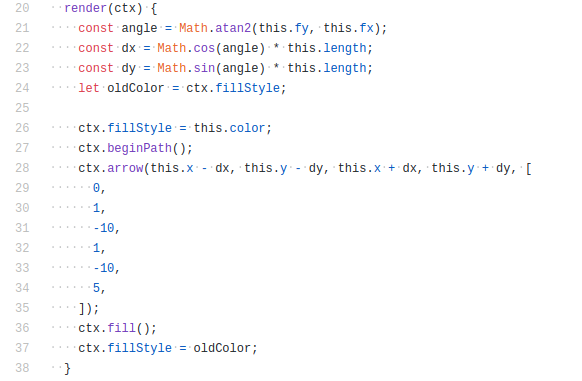
\includegraphics[scale=0.5]{img/vector_drawing.png}
        \caption{Funkcja rysująca wektor, kształt strzałki wyznaczany jest na bazie jej bazowej długości i kąta wektora siły. Implementacja wyznaczania siły używa metody calculate opisanej poniżej. Podmieniana jest jedynie pozycja krążka by zasymulować oddziaływanie w punkcie. }
        \label{fig:vector_drawing}
    \end{figure}
    
   \clearpage
   \item CoulombForce - klasa implementująca obliczenia modelu fizycznego. Oblicza przyspieszenie krążka na podstawie siły między dwoma przekazanymi ładunkami. Jej obiekt jest tworzony podczas dodawania ładunku w \emph{GameController} i dodawany do \emph{forces} w klasie \emph{Game}
 
  
    \begin{figure}[H]
    \centering
    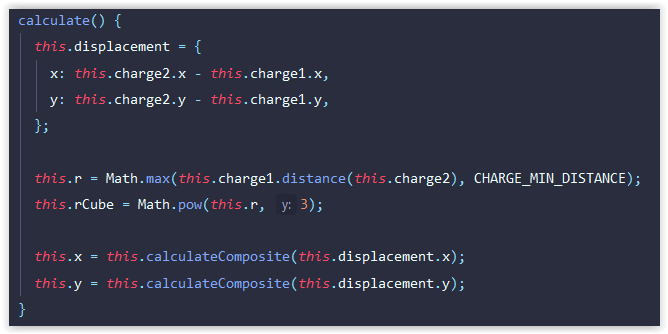
\includegraphics[scale=0.8]{img/Funkcja_calculate.PNG}

    \caption{Funkcja calculate obliczająca przyspieszenie krążka na podstawie siły między ładunkami}
    \label{fig:Funkcja_calculate}
    \end{figure}

\emph{calculate} - główna funkcja obliczająca przyspieszenie wypadkowe krążka, wykorzystywana w \emph{updateForces()} w \emph{Game}

\emph{displacement} przechowuje przemieszczenie między krążkiem a ładunkiem dla danych składowych

\emph{r} odległość między krążkiem a ładunkiem

\emph{rCube} odległość podniesiona do sześcianu, upraszcza obliczenia w\\
\emph{calculateComposite}

\emph{x,y} składowe wyznaczanej siły


\emph{calculateComposite()} funkcja oblicza przyspieszenie dla podanego przemieszczenia składowego. 
\\Odpowiednik w modelu fizycznym $$
a_{x}=k \cdot \frac{\sin \alpha}{m \cdot r^{2}} \quad a_{y}=k \cdot \frac{\cos \alpha}{m \cdot r^{2}}
$$
Odpowiednikiem sinusa lub cosinusa jest $\frac{\emph{displacement}}{r}$. Jako że w mianowniku występuje również $r^2$, wyrażenie $\frac{\emph{displacement}}{r \cdot r^2}$ zostało zastąpione przez $\frac{\emph{displacement}}{rCube}$

Czynniki \emph{charge.getSign()} w liczniku odpowiadają za wyznaczenie odpowiedniego kierunku przyspieszenia
    
    
\end{enumerate}

\subsection{Kontrollery}
\begin{enumerate}
    \item Controller - bazowa klasa dla pozostałych kontrolerów zawierająca pole \emph{eventBus} przechowujące obiekt klasy \emph{Eventbus} do obsługi zdarzeń w grze.
    
    \item InputController - klasa obsługująca zdarzenia wymuszone przez klienta przez funkcjonalności takie jak: przycisk, checkbox, pole typu 'input' i kliknęcia myszą. Dla każdego typu interakcji użytkownika z programem jest zaimplementowana jedna z funkcji \textit{registerButtonListeners(), registerCheckboxListeners(), registerRadioListeners(), registerInputListeners(), registerMouseListeners()} wysyłąjąca odpowiedni komunikat dzięki \emph{eventBus.emit()}.
    \item GameControler - klasa obsługująca wszelkie zdarzenia w grze.
    
    \emph{game} pole przechowujące aktualną sesję gry.
    
    \emph{registerListeners()} główna funkcja implementująca reakcję na konkretne zdarzenie wysłane przez grę lub użytkownika poprzez \emph{InputController}. Przez \emph{eventBus.on()} sprawdza czy aktywne jest dane zdarzenie
    
    \emph{clear()} wyczyszczenie planszy i stanu gry
    
    \emph{onDifficultyChange()} - funkcja reagująca na zmianę poziomu trudności
    
    \emph{placeCharge()} - funkcja obsługująca umiejscowienie ładunków na planszy
    
    \emph{showGoalMessageAnimation(), showFailureMessageAnimation()} - funkcje wyświetlające animacje tekstu w zależności od zdarzenia
    \end{enumerate}



\section{Literatura}
\begin{enumerate}
    \item Zbigniew Kąkol, Kamil Kutorasiński. Prawo Coulomba. 
    \item Zbigniew Kąkol. Fizyka. Kraków 2019
    \item David Halliday, Robert Resnick, Jearl Walker. Podstawy fizyki. Tom 3
\end{enumerate}

\end{document}

